\documentclass[11pt]{article}

\usepackage[margin=1in]{geometry}
\usepackage[T1]{fontenc}
\usepackage[utf8]{inputenc}
\usepackage{graphicx}
\usepackage[hidelinks]{hyperref}
\usepackage{enumitem}

\graphicspath{{../data/presentation_assets/}}
\setlist{noitemsep,topsep=1pt,leftmargin=1.15em}
\setlength{\parindent}{0pt}
\setlength{\parskip}{0.11em}

\title{\vspace{-2em}\textbf{What Really Makes a Pokemon Strong?}\\
\large Visualizing competitive success beyond raw stats}
\author{Team 13}
\date{}

\begin{document}
\maketitle
\vspace{-1.7em}

\section{Data and Story Focus}

Most people first judge Pokemon by stats. Our project asks whether that idea still works in competitive play. Our main claim is simple: raw stats matter, but competitive success also depends on teammates, usage, moves, items, abilities, and synergy.

The target audience is novice viewers. We will explain usage percentage as a proxy for competitive relevance, not perfect proof of strength. We define team connectivity degree as the number of unique teammate connections a Pokemon has in the cleaned co-usage network.

We use two Kaggle datasets. The Complete Competitive Pokemon Database (2022) provides VGC 2022 stats, usage, teammates, moves, items, abilities, and rules \cite{carbone2022competitive}. The 32000 Pokemon Images dataset provides sprites and metadata for visual identity \cite{singh32000pokemon}.

After cleaning, the data contains 1,098 Pokemon/form rows, 2,606 teammate co-usage edges, and 2,967 build usage rows. There are 228 Pokemon with numeric usage data. We also keep 32 rows with missing base stats and flag them for stat-based views.

The key finding starts the story. Total base stats and usage have a weak correlation of 0.194. Team connectivity degree and usage have a much stronger correlation of 0.903. So the project should not rank stat totals. It should show how Pokemon fit into teams. Zacian Crowned Sword has high stats and high usage. Zamazenta or Mewtwo show that high stats can still lead to low usage. Incineroar has moderate stats, but very high usage and team connectivity.

\begin{center}
  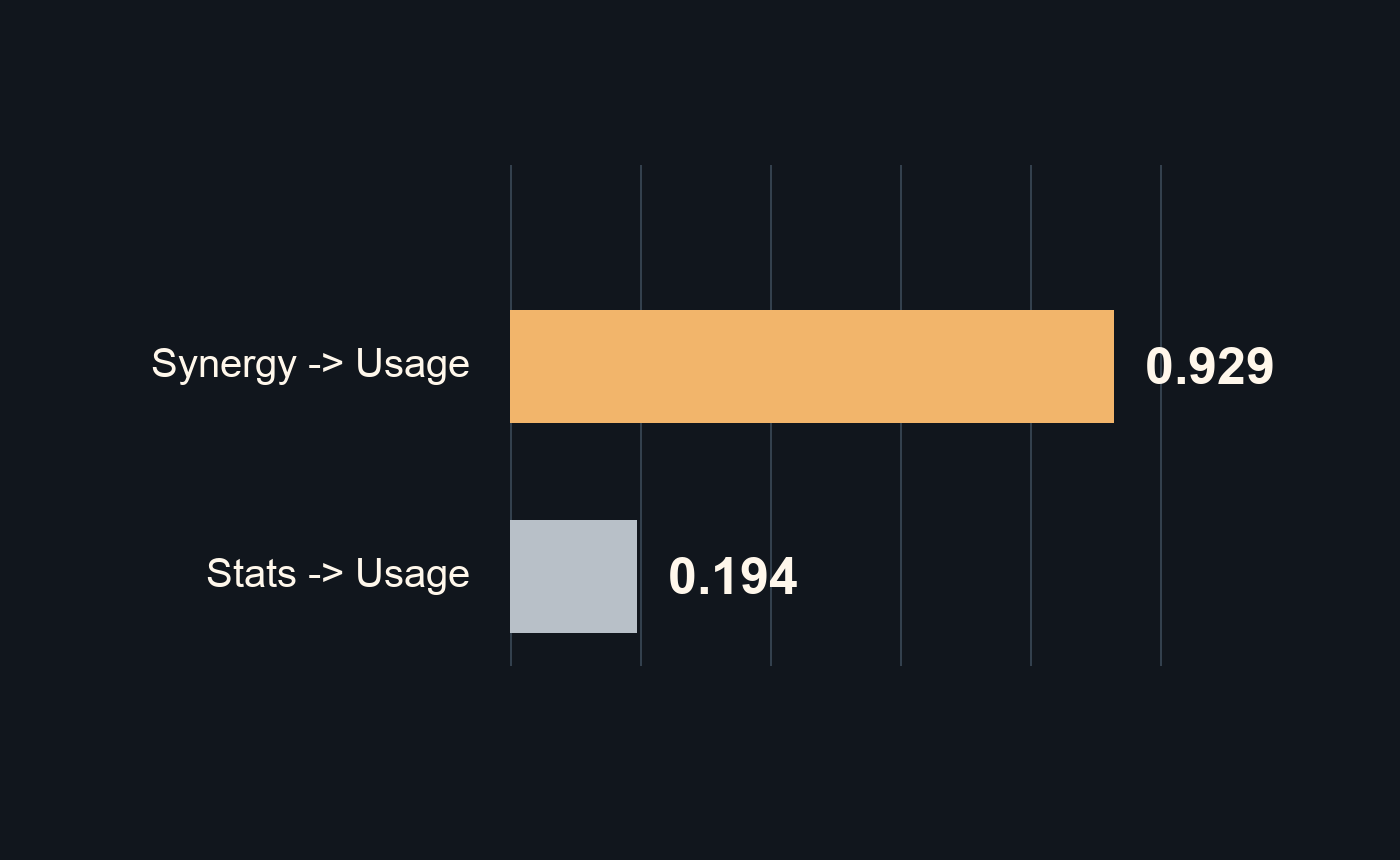
\includegraphics[width=0.52\linewidth]{correlation_insight.png}

  \small Figure 1. The story starts with a contradiction: stats weakly predict usage, while team connectivity is much more aligned with usage.
\end{center}
\vspace{-0.5em}

\section{Visualization Design}

The main visualization will be an interactive D3 force-directed team synergy network \cite{d3js}. This network is the main character of the story. Node means Pokemon. Edge means common teammate relationship. Larger node means higher usage. Thicker edge means stronger teammate co-usage. Node color shows primary type.

A network layout works well because competitive value is relational. Ordinary charts can show individual stats, but they cannot show how Pokemon fit into teams. The network reveals repeated teammate connections, which are the main point of the story.

Clicking a Pokemon will highlight its teammates and fade unrelated parts of the network. A detail panel will show image, type, total stats, usage, rank, top teammates, common moves, item, ability, and role. The goal is not to build a Pokedex browser. The goal is to show how team context explains competitive value.

\begin{center}
  \includegraphics[width=0.42\linewidth]{react_network_incineroar_cropped.png}

  \small Figure 2. Incineroar becomes central through repeated teammate connections, despite having lower raw stats than many legendary Pokemon.
\end{center}
\vspace{-0.5em}

Our drawing plan is staged. We first draw a small stats-vs-usage scatterplot to reveal the contradiction. Next, we draw three case-study cards or compact bars for Zacian, Zamazenta or Mewtwo, and Incineroar. Then we draw the force-directed network and start it with Incineroar selected. Cluster labels such as support connectors, legendary attackers, and weather/team cores will be added only to help viewers read the network. These are not dashboard panels, and the network remains the main visual focus.

React will handle page structure and selected state. D3 will handle scales, SVG drawing, and the force simulation \cite{react,d3js}.

\section{Storytelling Structure}

We choose a Martini Glass structure \cite{segel2010narrative}. The first part is guided. The viewer follows our argument step by step. After that, the network opens for exploration.

The story has five beats: start with the assumption that high stats mean strong Pokemon; use the stats-vs-usage scatterplot to show that it fails; use comparison cards or a small bar chart to introduce Zacian, Zamazenta or Mewtwo, and Incineroar; reveal the network with Incineroar selected; then let users click other Pokemon and explore team relationships.

The small views act as story steps, not dashboard panels. The scatterplot raises the question. The comparison cards or bar chart introduce the case-study Pokemon and show that attackers and support Pokemon can succeed for different reasons. Cluster and archetype labels help viewers read larger team patterns before open exploration. Together, these views guide attention toward the force-directed network, which remains the main character.

Text and annotations will guide attention at the beginning. One annotation can point to Incineroar: 530 total base stats, but many strong teammate connections. Thick edges will show repeated teammate pairings. The click interaction has drill-down behavior because users inspect one Pokemon at a time. But the overall story is Martini Glass because the user first follows a guided path before open exploration.

\newpage
\raggedright
\bibliographystyle{plain}
\bibliography{references}

\end{document}
